In this section let's give a short overview of related works that are based
onto the main results of~\cite{kolosov2016link} mainly on polynomials $\polynomialP{m}{b}{x}$.
\begin{figure}[H]
    \centering
    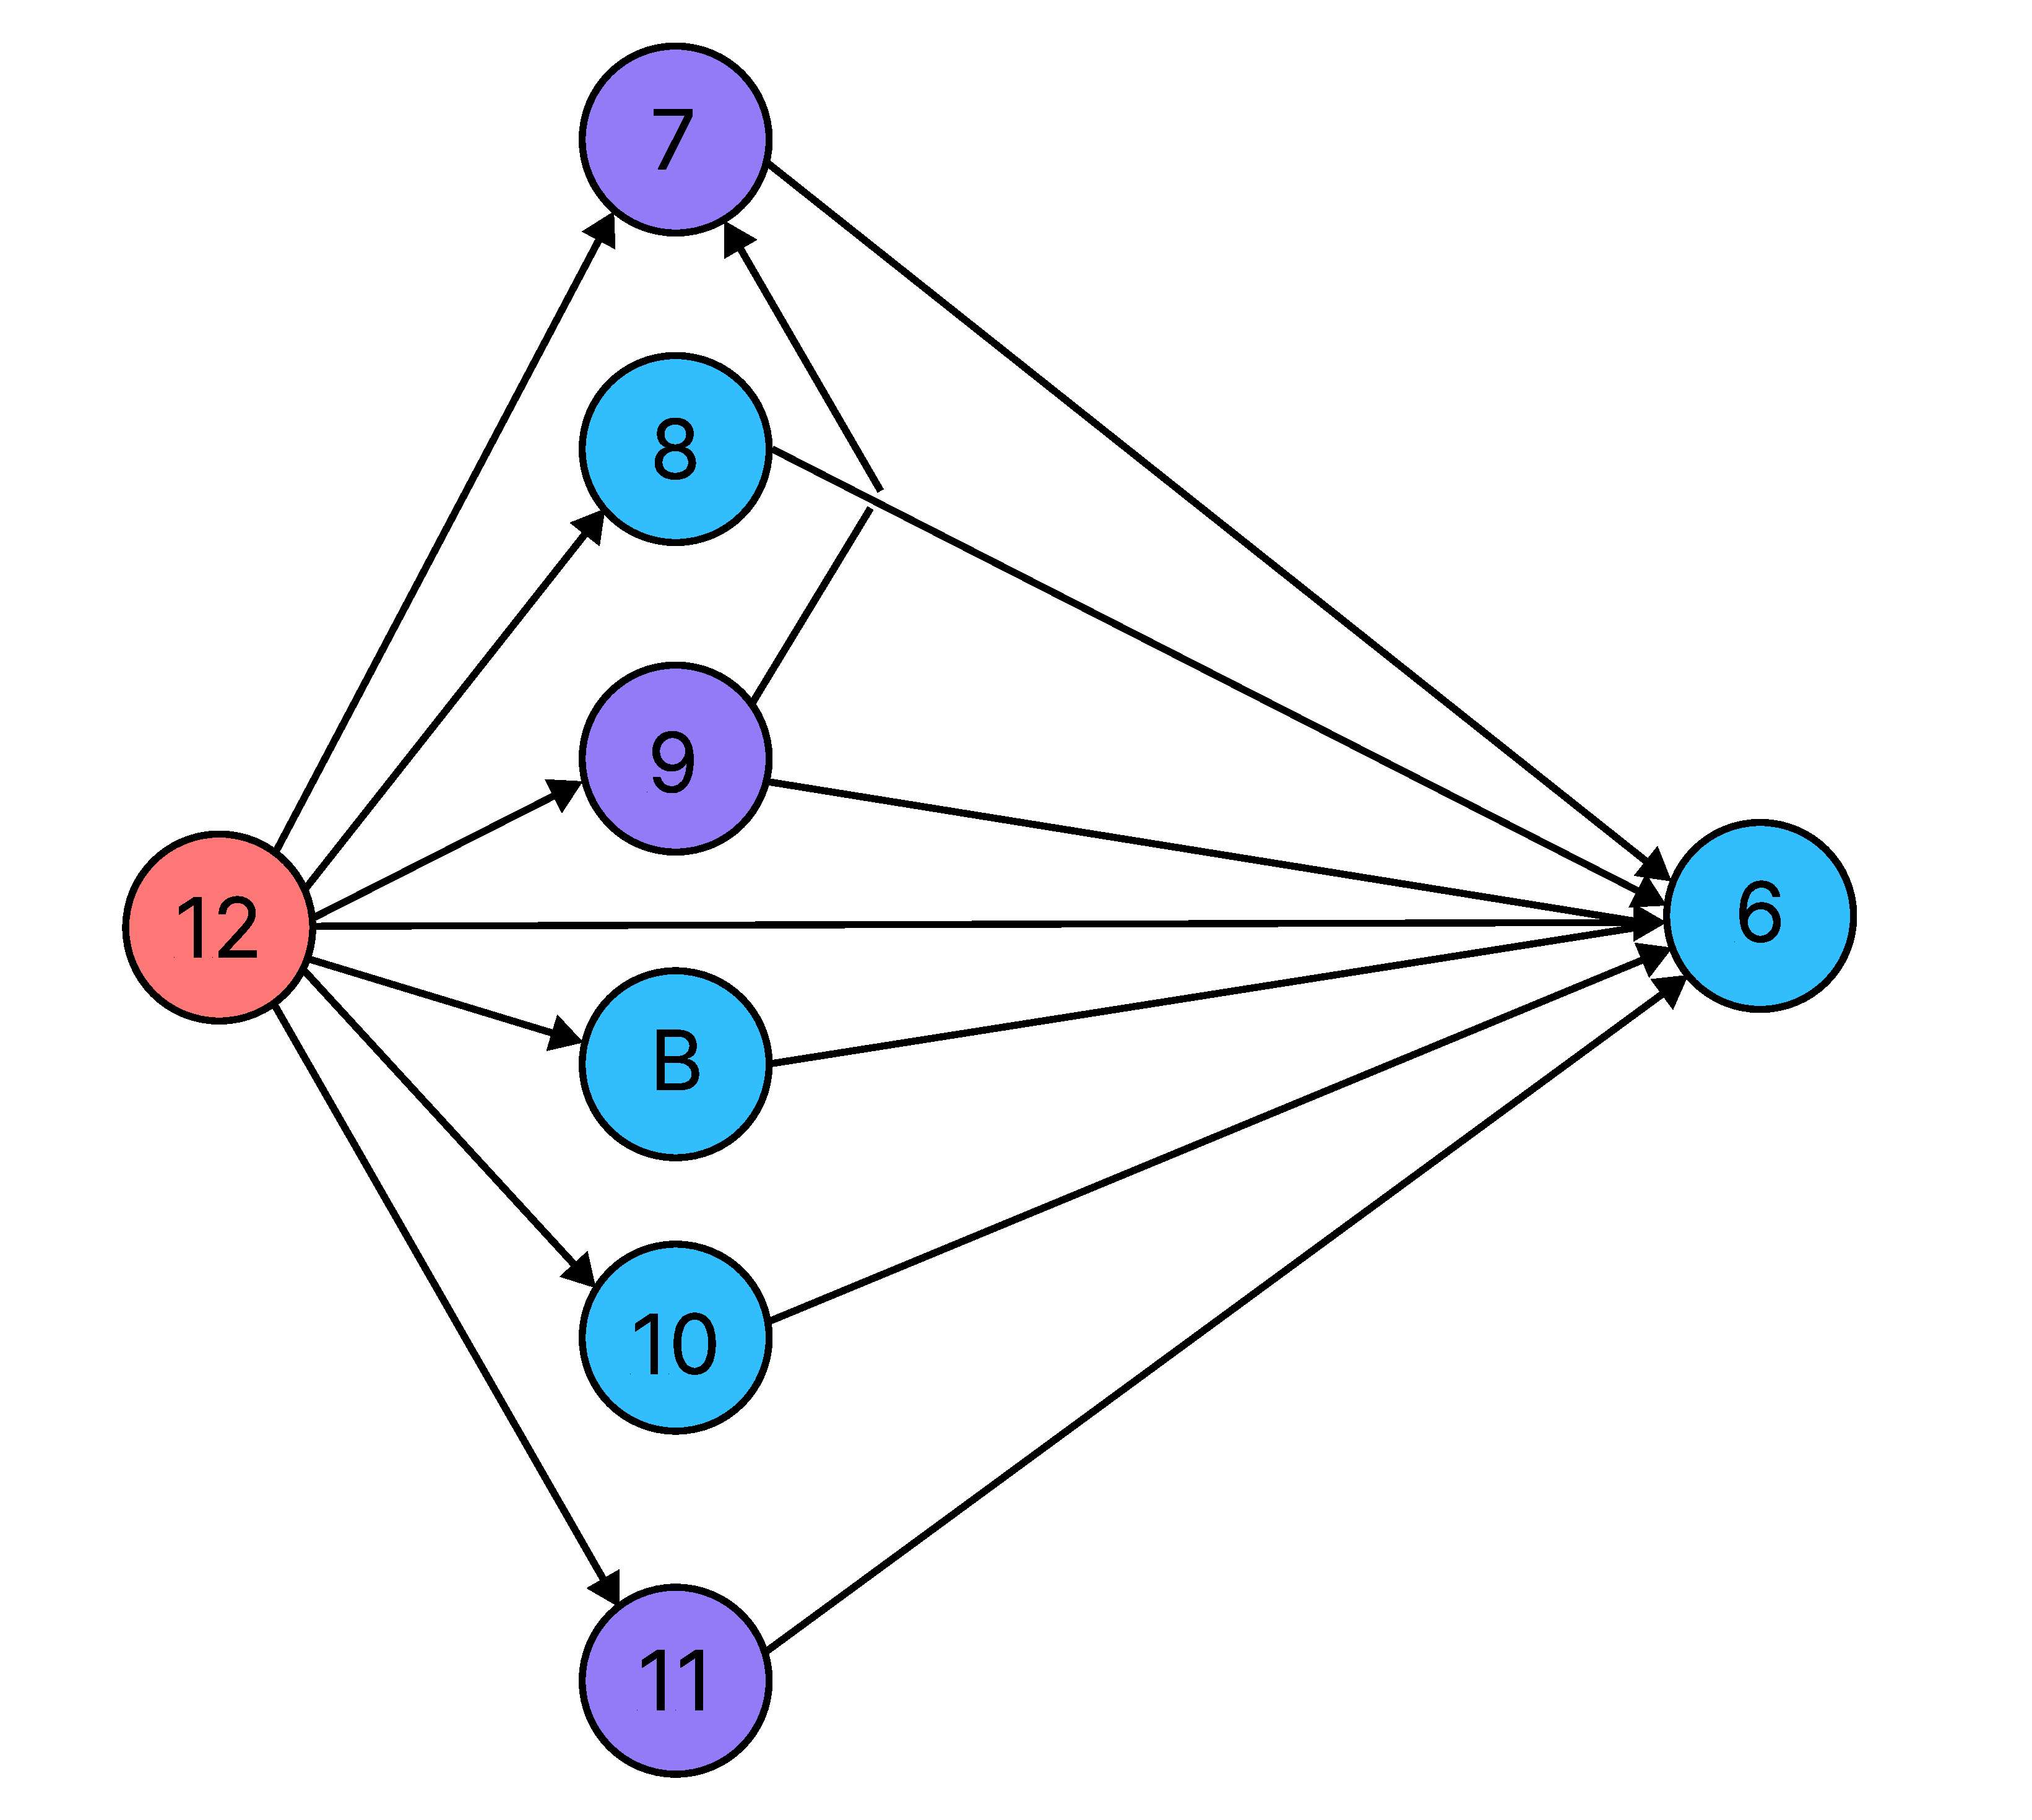
\includegraphics[width=1\textwidth]{images/realated_works_graph}
    ~\caption{Related works graph.}\label{fig:related-works-graph}
\end{figure}
\begin{itemize}
    \item In A study on partial dynamic equation on time scales involving derivatives
    of polynomials~\cite{kolosov2016study} which is denoted as 7:
    \item In 106.37 An unusual identity for odd-powers~\cite{kolosov2022106} which is denoted as 8:
    \item In Another approach to get derivative of odd-power~\cite{kolosov2023another} which is denoted as 9:
    is given a relation in terms of partial differential equations such that
    ordinary derivative of odd-power $2m+1$ can be reached in terms of partial derivatives of $\polynomialP{m}{b}{x}$.
    Let be a fixed point $v\in \mathbb{N}$, then ordinary derivative $\frac{d}{dx} g_v (u)$ of the odd-power function $g_v(x) = x^{2v + 1}$
    evaluate in point $u\in\mathbb{R}$ equals to partial derivative $(f_{v})^{'}_{x} (u, u)$ evaluate in point $(u, u)$ plus
    partial derivative $(f_{v})^{'}_{z} (u, u)$ evaluate in point $(u, u)$
    \begin{equation}
        \frac{d}{dx} g_v (u) = (f_{v})^{'}_{x} (u, u) + (f_{v})^{'}_{z} (u, u)
        \label{eq:odd-exponential-identity}
    \end{equation}
    where $f_{y} (x, z) = \sum_{k=1}^{z} \sum_{r=0}^{y} \coeffA{y}{r} k^r (x-k)^r = \polynomialP{y}{z}{x}$.
    Afterward, the equation~\eqref{eq:odd-exponential-identity}
    is generalized over the timescales $\mathbb{T} \times \mathbb{T}$ providing its dynamic equation analog
    in~\cite{kolosov2016study}.
    \item In Polynomial identity involving Binomial Theorem and Faulhaber's formula~\cite{kolosov2023polynomial}
    which is denoted as 10:
    \item In Finding the derivative of polynomials via double limit~\cite{kolosov_2024_10575485} which is denoted as 11:
    \item This manuscript is denoted as 12.


\end{itemize}

Second article~\cite{kolosov_2024_10575485} gives another perspective of ordinary derivatives of polynomials expressing
them via double limit as
\begin{align*}
    \lim_{h \to 0} \polynomialP{m}{x+h}{x} = x^{2m+1}
\end{align*}
that opens such opportunity.

In~\cite{barbero2020two} based on~\eqref{eq:equation7}, the authors give a new identity involving
Bernoulli polynomials and combinatorial numbers that provides,
in particular, the Faulhaber-like formula for sums of the form $1^m(n-1)^m + 2^m (n -2)^m + \cdots + (n - 1)^m 1^m$ for
positive integers $m$ and $n$.

Three sequences were contributed to
OEIS~\cite{kolosov2018coefficientspolynomial1, kolosov2018coefficientspolynomial2, kolosov2018coefficientspolynomial3}
showing the coefficients of the polynomial $\polynomialP{m}{b}{x}$ having fixed points $m,b$ while $x\in\mathbb{R}$.
